%%%%%%%%%%%%%%%%%%%%%%%%%%%%%%%%%%%%%%%%%%%%%%%%%%%%%%%%%%%%%%%%%%
%%%%%%%% ICML 2013 EXAMPLE LATEX SUBMISSION FILE %%%%%%%%%%%%%%%%%
%%%%%%%%%%%%%%%%%%%%%%%%%%%%%%%%%%%%%%%%%%%%%%%%%%%%%%%%%%%%%%%%%%

% Use the following line _only_ if you're still using LaTeX 2.09.
%\documentstyle[icml2013,epsf,natbib]{article}
% If you rely on Latex2e packages, like most moden people use this:
\documentclass{article}

% For figures
\usepackage{graphicx} % more modern
\usepackage{grffile}
%\usepackage{epsfig} % less modern
\usepackage{subfigure}
% For tables
\usepackage{booktabs}
\usepackage{multirow}
% For citations
\usepackage{natbib}
% For algorithms
\usepackage{algorithm}
\usepackage{algorithmic}
%utf-8 characters
\usepackage[T1]{fontenc}		% Selecao de codigos de fonte.
\usepackage[utf8]{inputenc}		% Codificacao do documento (conversão automática dos acentos)

% dummy text generator
\usepackage{blindtext}
% Comandos matemáticos
\usepackage{amsthm}
\usepackage{amsfonts}
\usepackage{amssymb}
\usepackage{amsmath}
\usepackage{MnSymbol}
\newtheorem{theorem}{\scshape Teorema}[section]
\newtheorem{teo}[theorem]{\scshape Teorema}
\newtheorem{lema}[theorem]{\scshape Lema}
\newtheorem{cor}[theorem]{\scshaé Corol\'ario}
\newtheorem{propo}[theorem]{\scshape Proposi\c{c}\~ao}
\newtheorem{definicao}{\scshape Defini\c{c}\~ao}[section]
\newtheorem{ex}{\scshape Exemplo}[section]
\newtheorem{obs}{Observação}[section]
\usepackage{listings}
\newcommand{\norm}[1]{\left\lVert#1\right\rVert}


%portuguese
%\usepackage[brazilian]{babel}

% For general purposes
\usepackage{indentfirst}
\setlength{\parindent}{1.3cm}
\setlength{\parskip}{0.2cm}

% As of 2011, we use the hyperref package to produce hyperlinks in the
% resulting PDF.  If this breaks your system, please commend out the
% following usepackage line and replace \usepackage{icml2013} with
% \usepackage[nohyperref]{icml2013} above.
\usepackage{hyperref}

% Packages hyperref and algorithmic misbehave sometimes.  We can fix
% this with the following command.
\newcommand{\theHalgorithm}{\arabic{algorithm}}

% Employ the following version of the ``usepackage'' statement for
% submitting the draft version of the paper for review.  This will set
% the note in the first column to ``Under review.  Do not distribute.''
\usepackage[accepted]{icml2013}
% Employ this version of the ``usepackage'' statement after the paper has
% been accepted, when creating the final version.  This will set the
% note in the first column to ``Proceedings of the...''
% \usepackage[accepted]{icml2013}


% The \icmltitle you define below is probably too long as a header.
% Therefore, a short form for the running title is supplied here:
\icmltitlerunning{Computer Vision and Tourist Attractions}

\begin{document}

\twocolumn[
\icmltitle{Computer Vision and Tourist Attractions}

% It is OKAY to include author information, even for blind
% submissions: the style file will automatically remove it for you
% unless you've provided the [accepted] option to the icml2013
% package.
\icmlauthor{Carlos Ronchi}{carloshvronchi@gmail.com}
\icmladdress{Universidade Federal do Paraná - UFPR}

% You may provide any keywords that you
% find helpful for describing your paper; these are used to populate
% the "keywords" metadata in the PDF but will not be shown in the document
\icmlkeywords{Machine learning, Computer Vision, cnn.}

\vskip 0.5in
]

\begin{abstract}
    Computer Vision has been achieving great advancements with the new
    state-of-the-arts algorithms, such as convolutional neural networks
    and its variants. With all these possibilities it's been possible
    to use images for cancer diagnosis \cite{Litjens} and recognizing
    places in geral \cite{places}. This current work intends to use convolutional
    neural networks and other models from machine learning to identify and predict
    some tourist attractions from the city of Curitiba, Brazil.
    This can be useful for tourists visiting the city and blind people who wants
    to know more about their surround.
\end{abstract}


\section{Introduction}

    The growing development of artificial inteligence (AI) allowed us to use images in the
    context of real world applications. One subfield of AI called Computer Vision, works
    towards developing technics in order to solve problems arising from images and videos
    for example.

    With such development, one can try to improve people's life using these algorithms.
    In that sense, one will implement convolutional neural networks and softmax
    regression to obtain a classifier of tourist atractions in Curitiba, which are
    the five following: The Cathedral Basilica Minor
    of Our Lady of Light, Botanical Garden, Oscar Niemeyer Museum, Wire Opera House,
    Paiol Theater.

\section{Softmax Regression}
  Given a dataset $\{(x^{(i)}, y^{(i)})\}_{i=1}^m$ with labeled data, that means
  $x^{(i)} \subset \mathbb{R}^n$ and $y^{(i)} \in \{1, \dots, k\}$ in the case of a
  multi-class problem. We want to try to predict a $\hat{y}_{i}$ such that it's
  close to $y^{(i)}$ given $x^{(i)}$ and a parameter $\theta \in \mathbb{R}^n$, which
  we do not know a prior. Instead of taking the sigmoid function which handles
  only the binary classification at once, consider the softmax function given
  in Equation \eqref{eq:softmaxeq}. In other words, given a test input $x$,
  we want our hypothesis to estimate the probability that $p(y=j|x)$ for
  each value $j=1,\dots,k$.

  \begin{equation}\label{eq:softmaxeq}
    \begin{split}
      m_{\theta}(x) &=
      \begin{bmatrix}
        p(y^{(i)}=1|x^{(i)}; \theta) \\
        p(y^{(i)}=2|x^{(i)}; \theta) \\
        \vdots                        \\
        p(y^{(i)}=k|x^{(i)}; \theta)
      \end{bmatrix}
      \\ &=
      \frac{1}{\sum_{j=1}^{k}e^{\theta_j^T x^{(i)}}}
      \begin{bmatrix}
        e^{\theta_1^T x^{(i)}} \\
        e^{\theta_2^T x^{(i)}} \\
        \vdots                \\
        e^{\theta_k^T x^{(i)}}
      \end{bmatrix},
    \end{split}
  \end{equation}
  where $\theta_1,\dots,\theta_k \in \mathbb{R}^n$ are the parameters of our model.
  Furthermore, notice that the sum $\frac{1}{\sum_{j=1}^{k}e^{\theta_j^T x^{(i)}}}
  $ normalizes the hypothesis vector, so that when one sums up the entries it'll
  give $1$.

  When using logistic regression, we tried to minimize the Equation \eqref{eq:logres}
  \begin{equation}\label{eq:logres}
    \begin{split}
      f(\theta) &= -\sum_{i=1}^{m} \Big[ y^{(i)}\log\left(m_\theta(x^{(i)})\right) \\
      &+ (1-y^{(i)}) \log\left(1-m_\theta(x^{(i)})\right) \Big],
    \end{split}
  \end{equation}
  with respect to the variable $\theta$. But since we changed our hypothesis function,
  we should consider the function given in Equation~\eqref{eq:costsoft} to be
  minimized.
  \begin{equation}\label{eq:costsoft}
    \begin{split}
      J(\theta) &= -\sum_{i=1}^{m} \sum_{j=1}^{k} 1_{y^{(i)}=j}
      \log \left( \frac{e^{\theta_j^T x^{(i)}}}{\sum_{l=1}^{k}e^{
      \theta_l^T x^{(i)}}} \right),
    \end{split}
  \end{equation}
  where $1_{y^{(i)}=j}$ is the indicator function, that means, if $y^{(i)} = j$,
  then $1_{y^{(i)}=j} = 1$, otherwise $1_{y^{(i)}=j}=0$. Note that if we
  consider $k=2$ and using some tricks we obtain logistic regression
  back.
  %For minimizing the function give in Equation~\eqref{label:costsoft} with
  %respect to the variable $\theta$, we may use descent methods, such

  Moreover, observe that $\theta$ is a matrix, whose column vectors are the
  parameters $\theta_1,\dots,\theta_k$ we are trying to adjust. In order
  to minimize the function~$J(\theta)$, we can use gradient descent methods, such
  as the steepest descent gradient, stochastic gradient descend, adam and
  many others.

  Taking derivatives, one can show that the gradient is
  \begin{equation}
    \nabla_{\theta_j} J(\theta) = \sum_{i=1}^{m}\Big[ x^{(i)}\left(
      1_{y^{(i)}=j} - p(y^{(i)}=j|x^{(i)})
    \right) \Big],
  \end{equation}
  where
  \begin{equation*}
    p(y^{(i)}=j|x^{(i)}) = \frac{e^{\theta_j^T x^{(i)
    }}}{\sum_{l=1}^{k}e^{\theta_l^T x^{(i)}}}.
  \end{equation*}
  And for example, using the gradient descent we would have the following
  rule for minimizing our function.
  \begin{equation*}
    \theta_j = \theta_j - \alpha \nabla_j J(\theta) \quad \forall j=1,\dots,k.
  \end{equation*}

\section{Deep Learning}
  Using neural networks with several stacked layers is called Deep Learning.
  These have been proven in the last few years to be very promising in the
  tasks of computer vision~\cite{ImageNet},~\cite{places}.

  Convolutional neural networks are a kind of neural
  networs with more operations instead of just using the vanilla
  $input\rightarrow activation \rightarrow output$. There are two fundamentals
  operations, the \emph{convolution}, hence convolutional neural networks and
  \emph{pooling}.
  The convolution layer takes as input an matrix, which can be 3d or not,
  and apply a certain number of filters (operations) over this matrix trying to
  find patterns. One such example is imagine one has a image of a square,
  and we apply the convolution with 4 filters of a certain size. They might
  find patterns, which will be in this case the four edges of a square.
  Roughly speaking, these filters are operating through matrix multiplications
  and sum of numbers.

  The pooling can be thought as a max pooling and average pooling, the well
  know poolings. A max pooling of size $s$ will take a sample of your image (as
  a matrix) and transform this square into a number, the maximum of the sample.
  And so one does over the whole image. The average pooling does the same, but
  instead of taking the maximum element in the sample we take the average.

\section{Data}

  Data has been collected web scrapping \emph{Google Images}. The Table~\ref{tab:nfiguras}
  shows the number of images collected and cleaned for
  the use of the algorithms.
  \begin{table}[htb]
      \centering
      \caption{Number of images from Tourist attractions.}
      \label{tab:nfiguras}
      \vskip 0.15in

      \begin{tabular}{@{}cc@{}}

      \toprule
        \textbf{Tourist Attraction}& \textbf{Number of Images}  \\
      \midrule
        Cathedral                  & 100                        \\
        Botanical Garden           & 171                        \\
        Museum                     & 92                         \\
        Wire Opera                 & 157                        \\
        Paiol Theater              & 73                         \\
      \bottomrule
      \end{tabular}
  \end{table}
  \begin{figure}[htb]
    \centering
    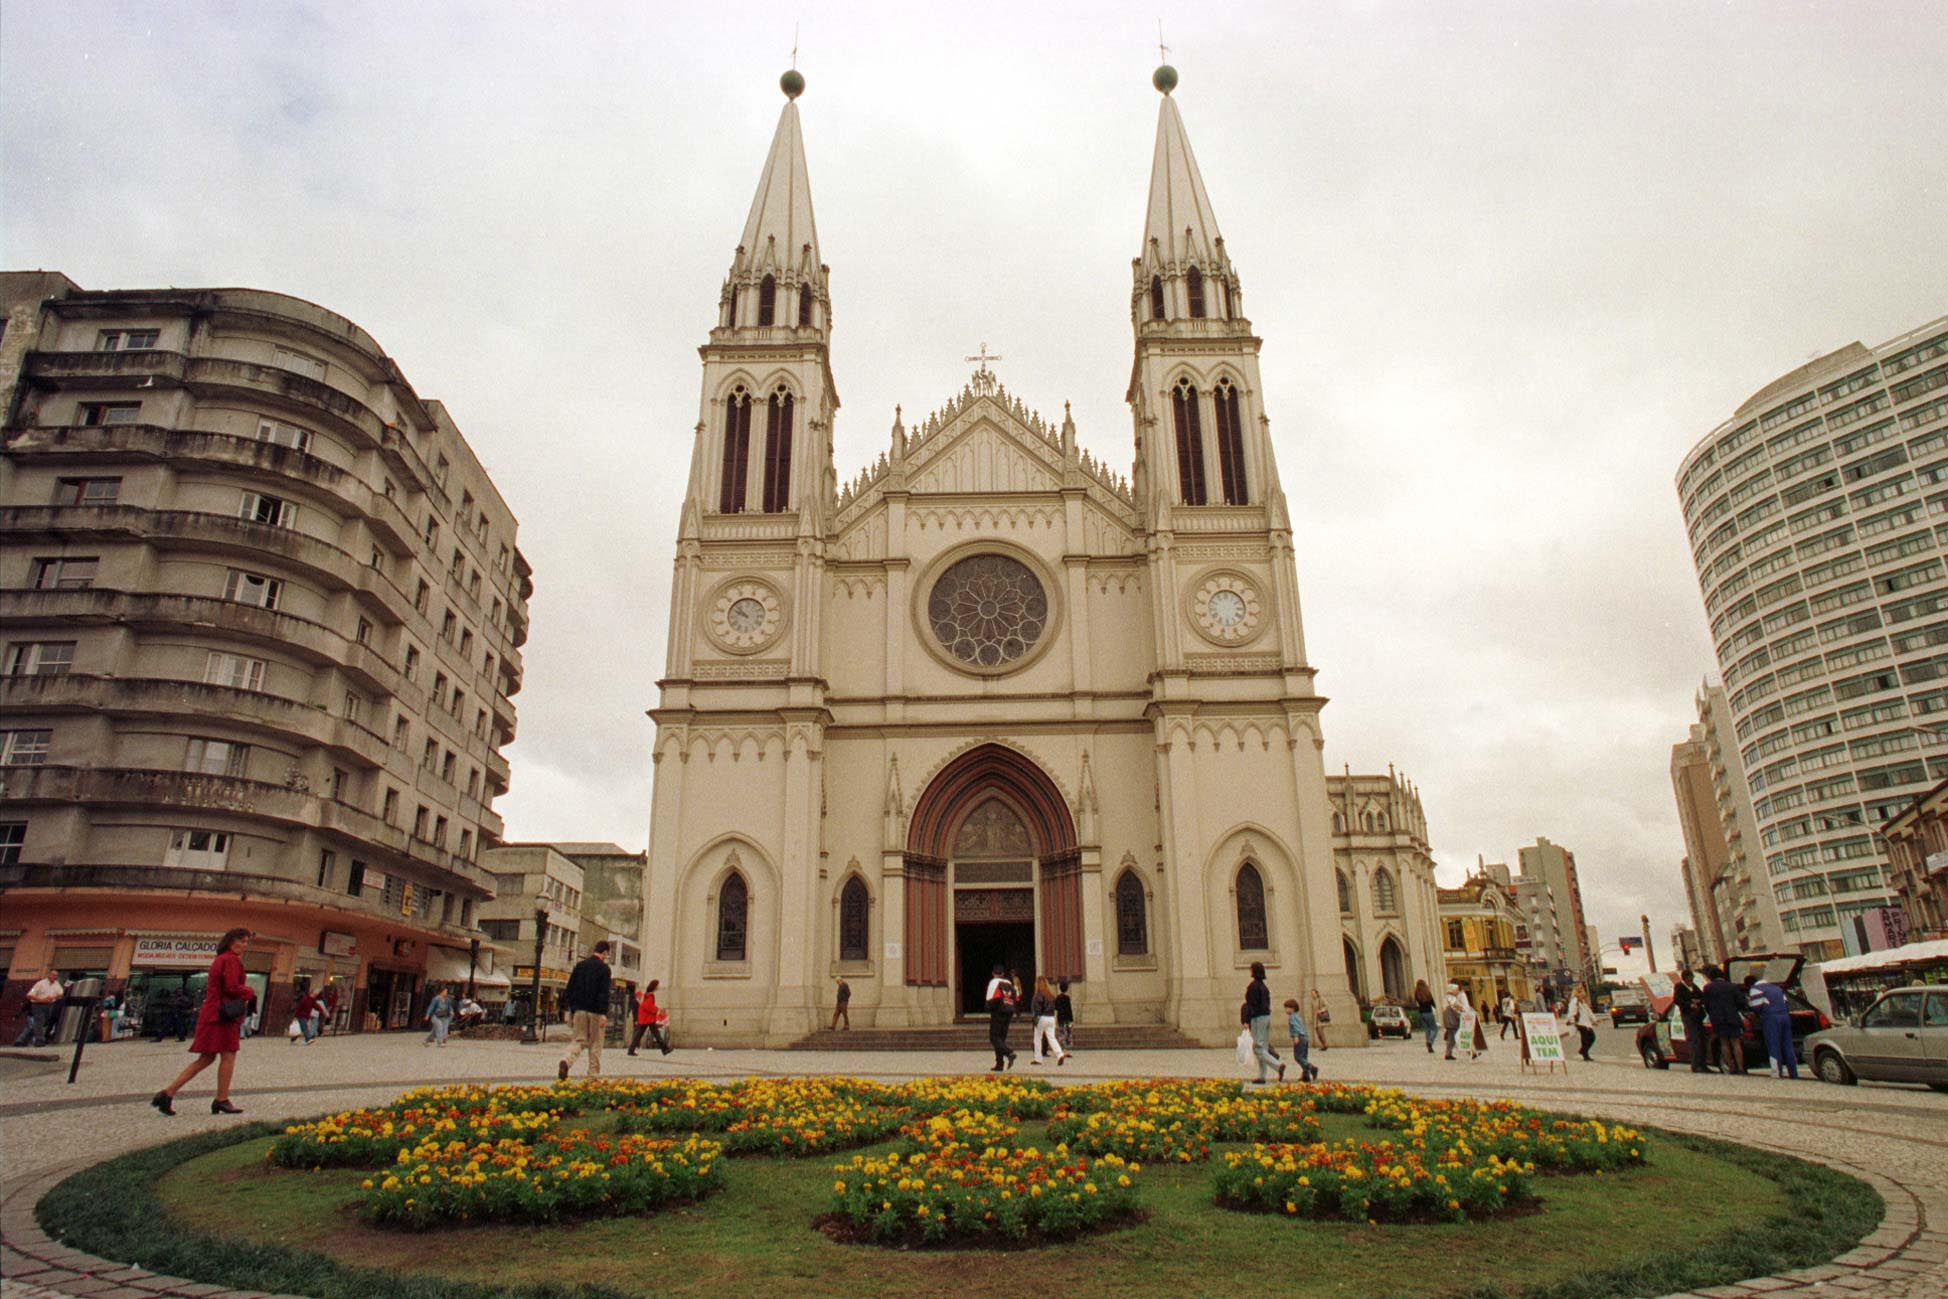
\includegraphics[width=0.45\textwidth]{0.jpg}
    \caption{Cathedral}
    \label{fig:0jpg}
  \end{figure}

  The pre-processing step for the images consisted in resizing the images to
  $224$px $\times$ $224$px.
  \begin{figure}[hbt]
    \centering
    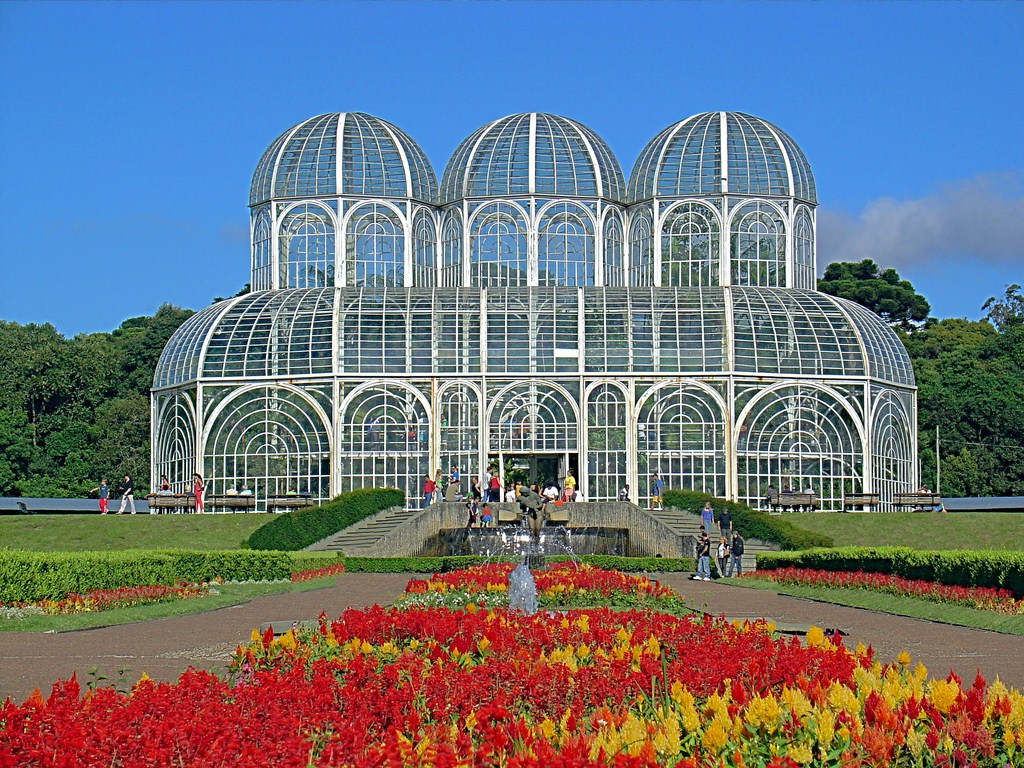
\includegraphics[width=.4\textwidth]{141.jpg}
    \caption{Botanical Garden}
  \end{figure}
\section{Implementation}
  It has been used the API from Google, \emph{TensorFlow}~\cite{tensorflow2015}
  to implement every algorithm.

  The algorithms implemented were the softmax regression and two kinds of
  convolutional neural networks. All implementations were made using Python and
  are available at \href{https://github.com/chronchi/CM116/Projeto}{Github}.

  For the deep learning models, two architectures were used, namely, a vanilla
  one given in TensorFlow's website and the other was based in the
  article~\cite{ImageNet}. The architectures are shown in Table~\ref{tab:archdeep}
  \begin{table}[hbt]
    \centering
    \caption{Architecture of the convolutional neural networks}
    \vskip 1.5mm
    \label{tab:archdeep}
    \begin{tabular}{|c|c|}
      \hline
      \multicolumn{2}{|c|}{ConvNet Configuration}     \\ \hline
      \textbf{Model 1}        & \textbf{Model 2}      \\ \hline
      4 weight layers         & 7 weight layers       \\ \hline
      \multicolumn{2}{|c|}{Input (224x224 RGB Image)} \\ \hline
      conv5-32                & conv11-64             \\ \hline
      \multicolumn{2}{|c|}{maxpool}                   \\ \hline
      conv6-32                & conv5-192             \\ \hline
      \multicolumn{2}{|c|}{maxpool}                   \\ \hline
      \multirow{3}{*}{}       & conv3-384             \\
                              & conv3-256             \\
                              & conv3-256             \\ \cline{2-2}
                              & maxpool               \\ \cline{2-2}
      FC1024                  & FC4096                \\
                              & FC4096                \\ \hline
      \multicolumn{2}{|c|}{Out}                       \\ \hline
      \multicolumn{2}{|c|}{Softmax}                   \\ \hline
    \end{tabular}
  \end{table}

  Here \textit{conv3-384} means that we are applying a convolutional
  layer using 384 filters each of size $3\times 3$.

  For the minimization of all functions it was used the Adam Optimizer~\cite{adam},
  whose routine is implemented in TensorFlow, and a mini batch rule for
  calculating the gradient, since the computer could not handle all the
  training examples at the same time. The mini batch sizes varied between
  10 to 220. It is important to notice that the activation function between
  the layers was ReLU, which is given on Equation~\eqref{eq:relu}
  \begin{equation}\label{eq:relu}
    f(x) = \max(0,x).
  \end{equation}
  For training the model it was used 80\% of the data and 20\% used for
  calculating the accuracy of the model.

\section{Results}
  Below in Table~\ref{tab:results} one can find the results for every model and
  with the number of classes used for that specific model. The values in each sell
  represent the accuracy of the model calculated on the test set.
  \begin{table}[htb]
    \centering
    \caption{Accuracy for every model for every number of classes.}
    \vskip 2mm
    \label{tab:results}
    \begin{tabular}{@{}cccc@{}}
      \toprule
      \textbf{\#Classes}        & \textbf{Model 1} & \textbf{Model 2} & \textbf{Softmax} \\
      \midrule
      2                         & $65,38\%$        & $88,46\%$        & $75\%$           \\
      3                         & -                & $80\%$           & $69,23\%$        \\
      4                         & -                & $71,84\%$        & $65,05\%$        \\
      5                         & -                & $75,83\%$        & $63,33\%$        \\
      \bottomrule
    \end{tabular}
  \end{table}

  As can be seen above, the first model did not perform so well, this might
  be happening because it is a shallow neural network, thus can not learn
  many parameters fully. In light of that, it was chosen that the
  architecture of model 1 was no to not use for further training new models.

  Notice that the Softmax and Model 2 achieved almost the same accuracy, eventhough
  the running time for the Model 2 was much bigger (around 2 hours), while
  for the softmax was under 10min.

  In the case of five classes, the perfomance of Model 2 was much better than the
  softmax, mainly because it can learn more parameters, it's more deep and complex
  than a softmax model.

  When Classes $= 3$, observe the Figure~\ref{fig:errorsoft}, as one can notice,
  the softmax error (upper plot) became less noisy with fewer steps than alexnet does,
  this might happens since alexnet is deeper and more complex in order to learn.
  \begin{figure}[htb]
    \centering
    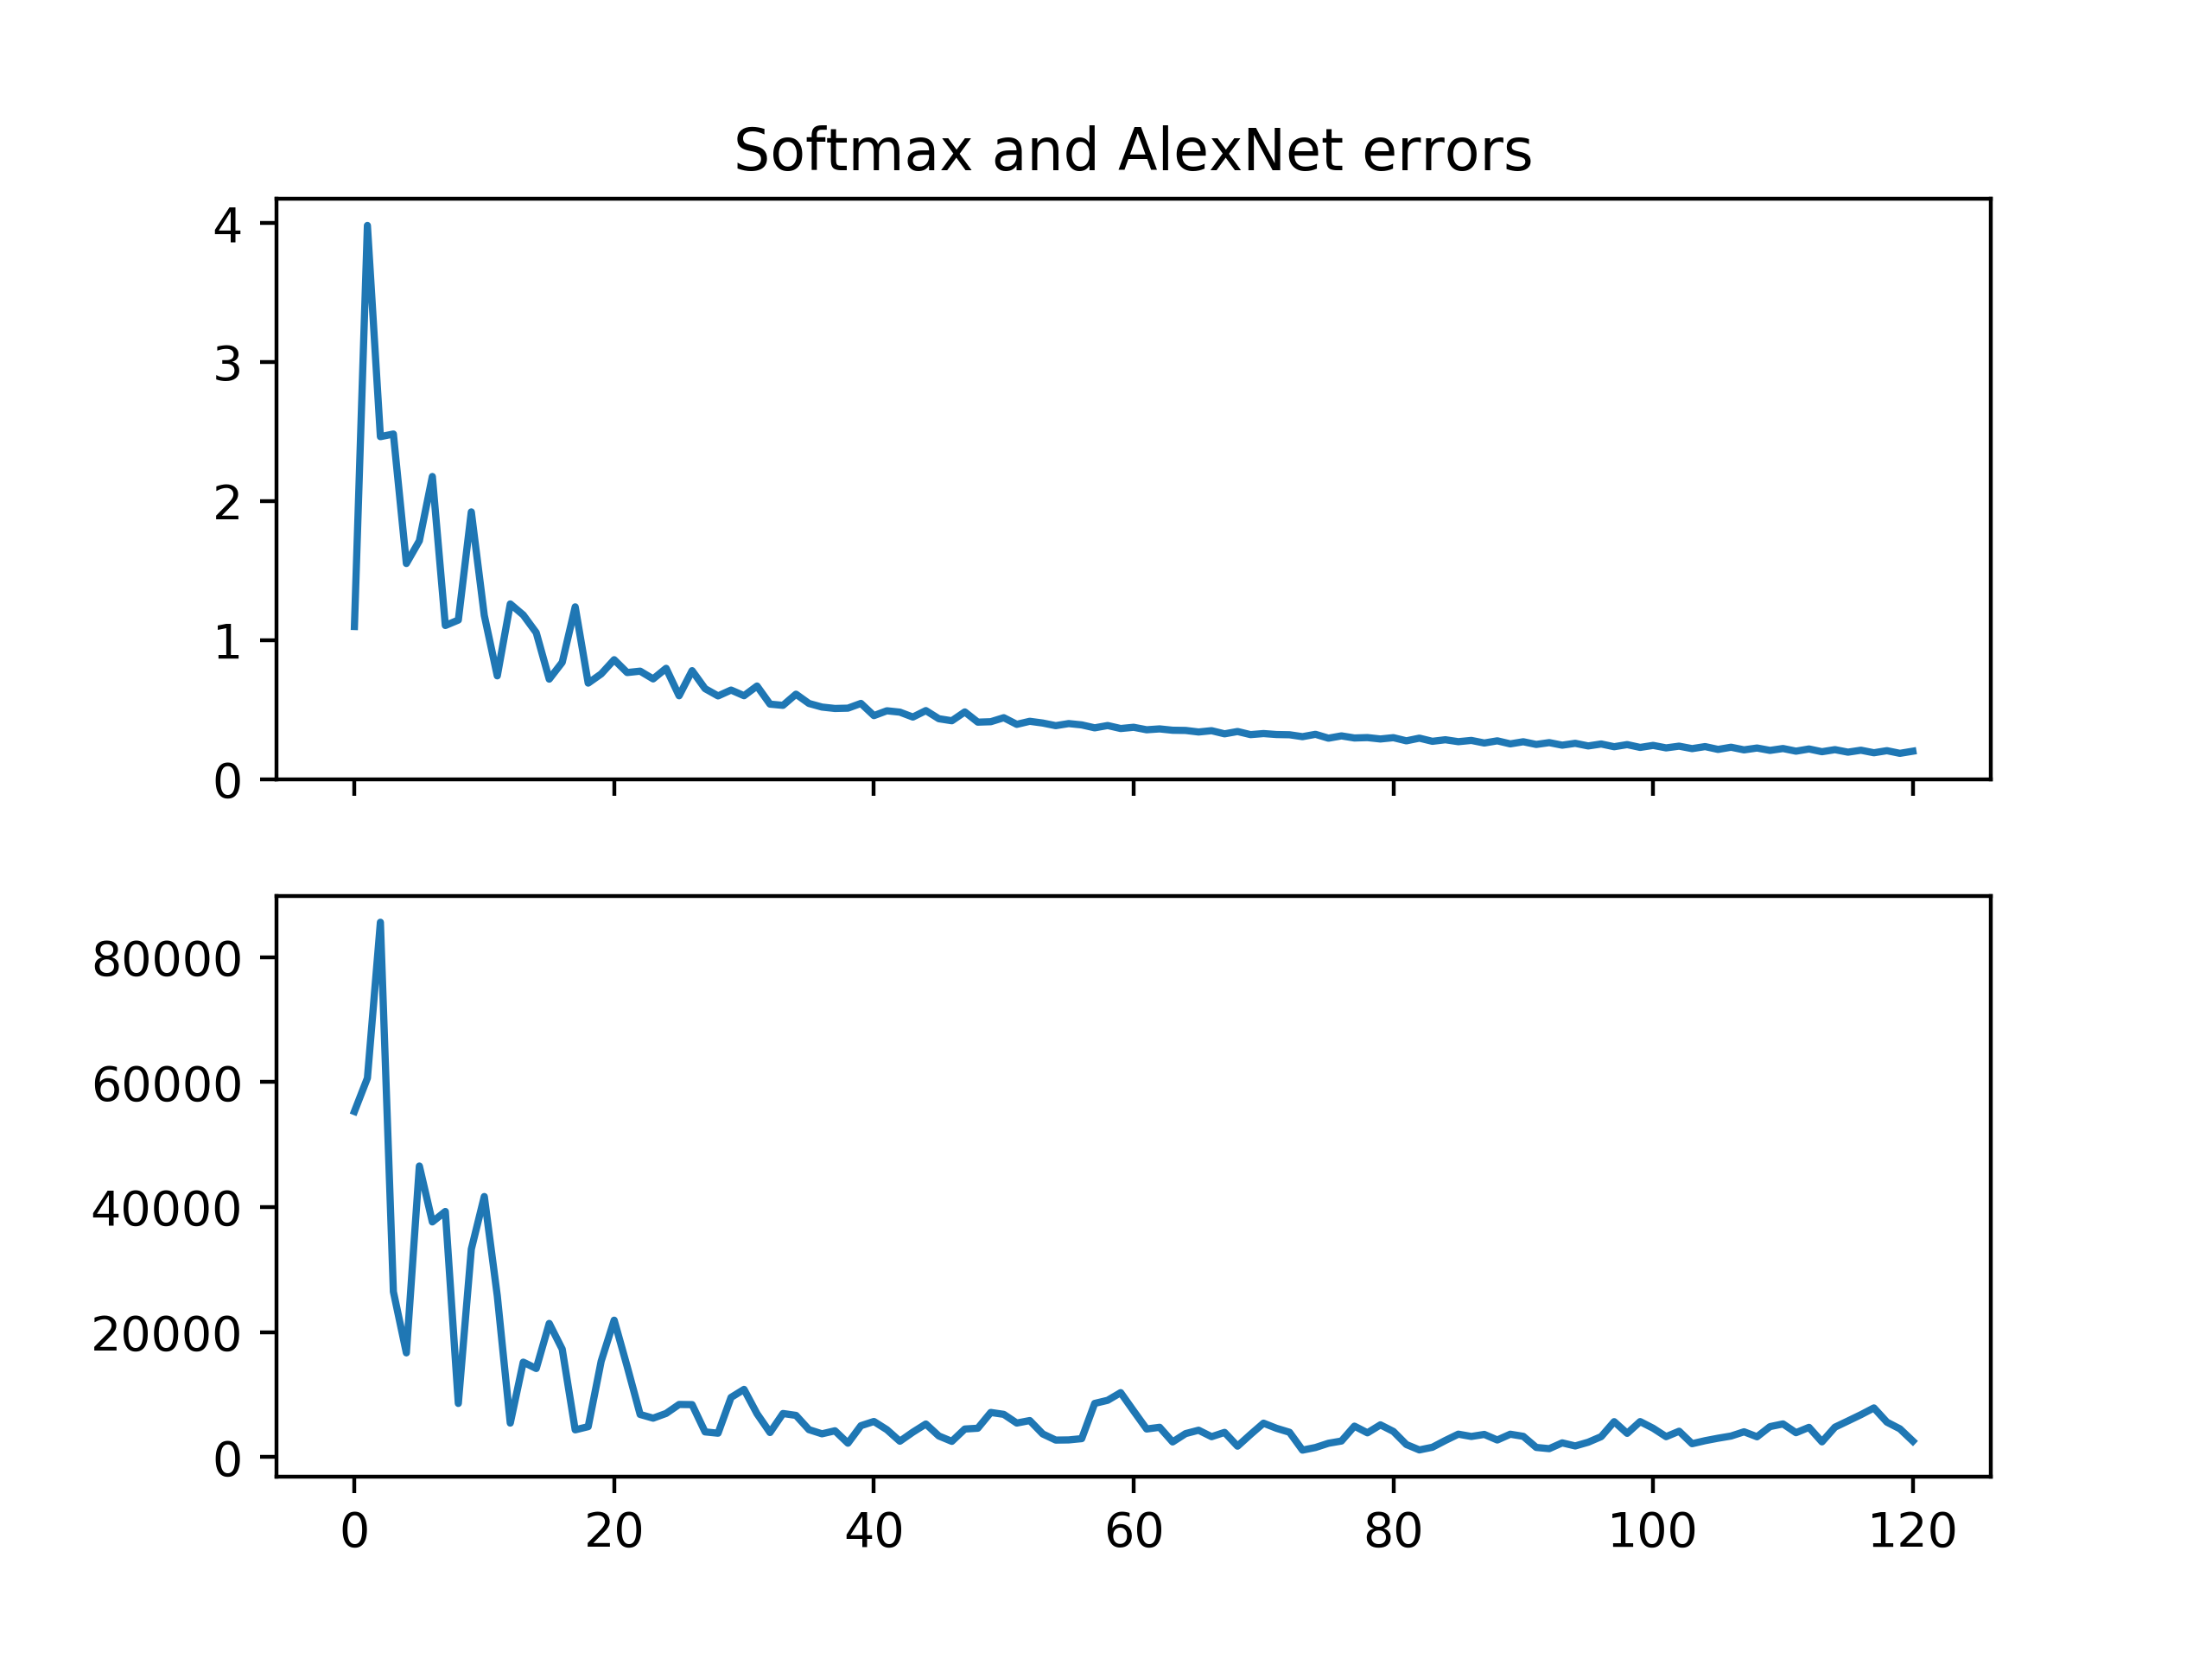
\includegraphics[width=.48\textwidth]{errors.png}
    \caption{Erros calculated on mini-batchs during training. Softmax error
    (upper image) and alexnet error (lower image).}
    \label{fig:errorsoft}
  \end{figure}

\section{Conclusion}
  The results obtained showed that CNN's can achieve better results than
  softmax regression. Furthermore, it might be possible to train this model
  with more classes given more data. The models learnt well enough
  considering that data was scarce.

\section{Future work}
  This work can be extended using newer convolutional neural networks, such
  as VGG16~\cite{vgg16}, Inception by Google~\cite{inception} and GAN~\cite{
  gan}.

  Another way for improving the results is adding pre-processing steps, such as
  taking the mean from the training set, autoencoders, which are neural networks
  with one small hidden layer and the output has the same size as input. Other
  way of improving it is using the CNN's as feature extractors and linking
  them as inputs to a linear SVM.

  Images are very important in this process, so to further improve the results
  it is necessary to obtain more data, perhaps through a web pipeline where
  people upload pictures and open sourcing this project. Other way would be
  artificially increasing the dataset using data augmentation.

\bibliography{ref}
\bibliographystyle{bibstylenew}

\end{document}
